%!TEX root = labo.tex

\setcounter {chapter} {5} 

\chapter{LAN switching}

What you will learn in this lab:
\begin{itemize}
	\item How to configure a Cisco Router and a Linux PC as a LAN switch.
	\item How LAN switches update their forwarding tables.
	\item How LAN switches run a spanning tree protocol for loop free routing.
\end{itemize}

\newpage
\setsession{prelab6}
\section{Prelab 6}\label{sec:prelab6}
%!TEX root = labo.tex

\subsubsection*{Bridges and the Spanning Tree Protocol}
Use the following resources to prepare yourself for this lab session:
\begin{enumerate}
	\item Bridging: Read about LAN switching and bridging at \url{http://docwiki.cisco.com/wiki/Internetworking_Technology_Handbook#Bridging_and_Switching}.
	\item Transparent Bridges and Spanning Tree Protocol: Read about transparent bridges and the spanning tree protocol at \url{http://docwiki.cisco.com/wiki/Transparent_Bridging}.
	\item Bridge Protocol Data Unit (BPDU): Familiarize yourself with the format of bridge protocol data units (BPDUs) by reading the information at \url{http://ericleahy.com/index.php/implementing-spanning-tree-protocol-stp/}.
	\item Configuring a PC as a Bridge: Explore the website \url{http://www.linuxfoundation.org/collaborate/workgroups/networking/bridge}, which describes the bridge-utils software package for configuring a Linux PC as a bridge.
\end{enumerate}

\newpage
\subsection*{Prelab Questions}
\begin{questions}
	\q{1}{Describe the difference between a LAN switch/bridge and a router?}
	\q{2}{What is the difference between an Ethernet switch and an Ethernet hub? Which is more suitable for a network with a high traffic load, a switch or a hub? Explain.}
	\q{3}{What motivates the use of the term "transparent" in transparent bridges?}
	\q{4}{Which role does the spanning tree protocol play when interconnecting LAN switches/bridges?}
	\q{5.a}{In the context of the IEEE 802.1d specification of the spanning tree protocol, define root bridge.}
	\q{5.b}{In the context of the IEEE 802.1d specification of the spanning tree protocol, define root port.}
	\q{5.c}{In the context of the IEEE 802.1d specification of the spanning tree protocol, define designated bridge.}
	\q{5.d}{In the context of the IEEE 802.1d specification of the spanning tree protocol, define designated port.}
	\q{5.e}{In the context of the IEEE 802.1d specification of the spanning tree protocol, define blocked port.}
	\q{6}{In the spanning tree protocol, how does a LAN switch/bridge decide which ports are in a blocking state?}
\end{questions}


\newpage
\setsession{lab6}
\section{Lab 6}\label{sec:lab6}

A bridge or LAN switch is a device that interconnects two or more Local Area Networks (LANs) and forwards packets between these networks. Different from IP routers, bridges and LAN switches operate at the data link layer. For example, bridges and LAN switches forward packets based on MAC addresses, whereas IP routers forward packets based on IP addresses.

LAN switches are widely deployed in enterprise networks, including university campus networks. Many enterprise networks primarily use LAN switches, and use IP routers only to connect the enterprise network to the public Internet.

The term 'bridge' was coined in the early 1980s. Today, when referring to data-link layer interconnection devices, the terms 'LAN switch' or 'Ethernet switch' (in the context of Ethernet) are much more common. Since many of the concepts, configuration commands, and protocols for LAN switches in Lab 6 use the old term 'bridge', we will, with few exceptions, refer to LAN switches as bridges.

This lab covers the main concepts of LAN switching in Ethernet networks: how packets are forwarded between LANs and how the routes of packets are determined. In the first and second parts of Lab 6, you learn how to configure a Linux PC and a Cisco router as a bridge. The third part illustrates the difference between an Ethernet hub and an Ethernet switch. Parts 4 explores how forwarding tables of bridges are set up. You learn about the concepts of learning bridges and transparent bridges.

The configuration of the equipment in Lab 6 is changed several times during the course of the lab. With exception of the last part, the IP address configuration of the Linux PCs is as shown in Table \ref{tab:lab6-network1}. Note that all IP addresses have the same netmask.

\begin{table}[h!t]
\centering
	\begin{tabular}{| c | c | c |}	
		\hline
		\textbf{Linux PC} & \textbf{eth0} & \textbf{eth1} \\ \hline
		PC1 & 10.0.1.11/24 & 10.0.1.12/24 \\ 
		PC2 & 10.0.2.21/24 & 10.0.1.22/24 \\
		PC3 & 10.0.3.31/24 & 10.0.1.32/24 \\
		PC4 & 10.0.4.41/24 & 10.0.1.42/24 \\ \hline
	\end{tabular}
	\caption{IP addresses}
	\label{tab:lab6-network1}
\end{table}

\newpage
\subsection{Configuring a Linux PC as a bridge}

The exercises in this lab show how to configure a Linux PC as a bridge. Ethernet bridging functionality is integrated in all recent versions of Linux. The configuration of bridging functions in Linux is done with configuration commands and tools. In this lab, we use the command-line bridge configuration tool \cmd{brctl}.

The network configuration for this part is shown in Figure \ref{fig:lab6-network1}. Here, PC1 and PC3 act as hosts and PC2 is set up as a bridge.

\begin{figure}[h!t]
	\centering
	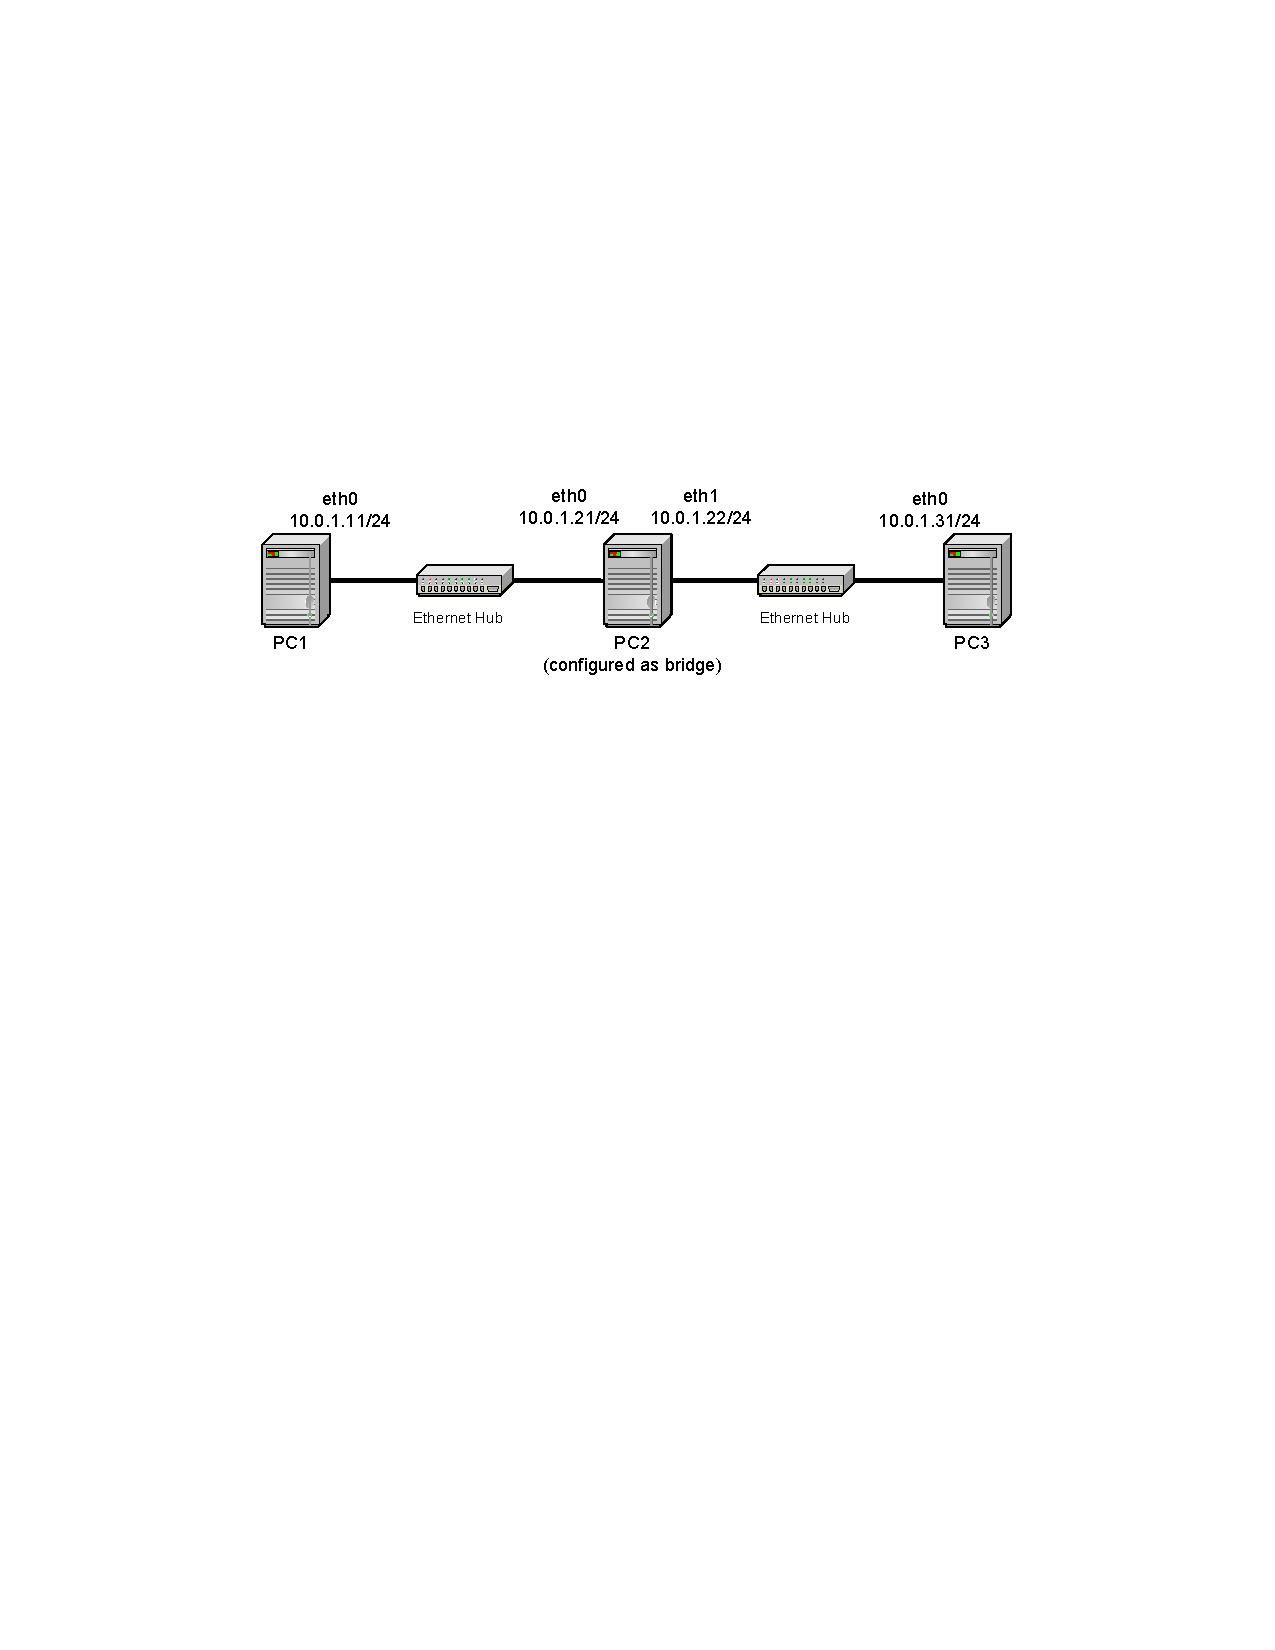
\includegraphics[width=\linewidth]{graphics/lab6-network1.pdf}	
	\caption{Network Topology for Part 1.}
	\label{fig:lab6-network1}
\end{figure}

\subsubsection{Exercise 1-a. IP configuration of Linux PCs}
\begin{enumerate}
	\item Set up the network configuration as shown in Figure \ref{fig:lab6-network1}.
	\item Configure the interfaces of PC1, PC2, and PC3, with the IP addresses given in Table \ref{tab:lab6-network1}. Disable the interfaces that are not used in the configuration, that is, disable interface \iface{eth1} on both PC1 and PC3.
	\item Since, throughout Lab 6, you frequently work with MAC addresses, you should record the MAC addresses of the Linux PCs. Log in to each of the PCs and obtain the MAC addresses of both Ethernet interfaces with the command \cmd{ifconfig -a}. Enter the MAC addresses in Table \ref{tab:lab6-macs-pcs}. (In Part 2, you will repeat the same exercise on the Cisco routers.)
		\begin{table}[h!t]
			\centering
			\begin{tabular}{| c | c | c |}	
				\hline
				\textbf{Linux PC} & \textbf{MAC address of eth0} & \textbf{MAC address of eth1} \\ \hline
				PC1 & 68:05:ca:36:33:a0 & 68:05:ca:39:cc:79 \\ 
				PC2 & 68:05:ca:36:31:f0 & 68:05:ca:39:e1:36 \\
				PC3 & 68:05:ca:36:39:c7 & 68:05:ca:36:51:3f \\
				PC4 & 68:05:ca:39:e1:2f & 68:05:ca:39:e1:32 \\ \hline
			\end{tabular}
			\caption{MAC addresses of the linux PCs}
			\label{tab:lab6-macs-pcs}
		\end{table}
\end{enumerate}

\subsubsection{Exercise 1-b. Configure a Linux PC as a bridge}
In this exercise, you configure PC2 as a bridge that forwards packets between the two Ethernet segments shown in Figure \ref{fig:lab6-network1}. The bridge configuration on the Linux PCs is done with the tool \cmd{brctl}.
\begin{enumerate}
	\item Creating a bridge with \cmd{brctl}: It is possible to configure multiple independently operating bridges on the same PC. Each bridge is assigned a name and is associated with a set of interfaces. Here, you configure one bridge on PC2 and assign the bridge the name Bridge1.
		\begin{cmdblock}
	brctl addbr Bridge1	
		\end{cmdblock}
		Check if the bridge has been created by typing:
		\begin{cmdblock}
	brctl show
		\end{cmdblock}
	\item Configuring a bridge with \cmd{brctl}: After the bridge is created, the bridge is configured in the following steps:
		\begin{itemize}
			\item Assign interfaces to the bridge. e.g. for PC2, add the interfaces \iface{eth0} and \iface{eth1}.
				\begin{cmdblock}
	brctl addif Bridge1 eth0
	brctl addif Bridge1 eth1
				\end{cmdblock}
			\item The next part of the configuration sets the parameters of the spanning tree protocol (STP). In Part 1, the spanning tree protocol is not used. Therefore, you need to disable the spanning tree protocol by toggling the button next to the STP label, so that it shows the label Disabled.
				\begin{cmdblock}
	brctl stp Bridge1 off
				\end{cmdblock}
			\item In the last part of the bridge configuration, you activate the bridge \iface{Bridge1} from a terminal window. On a Linux PC, each created bridge is represented as a network interface. Therefore, if you type the command ifconfig -a on PC2, the command shows an interface Bridge1, in addition to the other interfaces \iface{eth0}, \iface{eth1}, and \iface{lo}. The bridge is activated by enabling the interface associated with the bridge. This is done with the following command:
				\begin{cmdblock}
	PC1% ifconfig Bridge1 up
			\end{cmdblock}
			\boxwarning{Activating the bridge disables the IP configuration of the interfaces assigned to a bridge. Hence, it is no longer possible to issue ping commands to these interfaces.}
		\end{itemize}
\end{enumerate}

\boxinfo{The following settings can also be configured on a bridge interface. You don't need to change them for this exercise however.
	\begin{description}
		\item[\texttt{setageing <bridge> <time>}] \hfill \\
			Set ageing time to <time> for bridge interface \iface{<bridge>}
		\item[\texttt{setbridgeprio <bridge> <prio>}] \hfill \\
			Set bridge priority to <prio> for bridge interface \iface{<bridge>}
		\item[\texttt{setfd <bridge> <time>}] \hfill \\
			Set bridge forward delay to <time> for bridge interface \iface{<bridge>}
		\item[\texttt{sethello <bridge> <time>}] \hfill \\
			Set hello time to <time> for bridge interface \iface{<bridge>}
		\item[\texttt{setmaxage <bridge> <time>}] \hfill \\
			Set the maximum message age to <time> for bridge interface \iface{<bridge>}
		\item[\texttt{stp <bridge> {on|off}}] \hfill \\
			Turn the Spanning Tree Protocol on/off for bridge interface \iface{bridge}
	\end{description}
}


\subsubsection{Exercise 1-c. Observing a bridge in operation}
\boxwarning{You will use Wireshark in this exercise. Do not forget to append the binary dump (pcap format) to your lab report}

When the bridge configuration of PC2 is complete, PC2 forwards packets between PC1 and PC3. This exercise asks you to observe the forwarding.
\begin{enumerate}
	\item Start Wireshark on PC1 and PC3, and capture traffic on interface \iface{eth0} on both systems.
	\item When bridging is activated on PC2, the configured IP addresses on PC2 should be disabled. To verify this, issue a ping command to interfaces \iface{eth0} and \iface{eth1} of PC2 from PC1 and PC3.
		\begin{cmdblock}
	PC1% ping 10.0.1.21
	PC3% ping 10.0.1.22
		\end{cmdblock}
		If PC2 is configured as a bridge, these ping commands should fail.
	\item Clear the ARP caches on PC1 and PC3. Note that in Linux, each ARP entry has to be deleted separately with the command \cmd{arp -d <MACaddress>}.
	\item Issue a ping command from PC1 to PC3 and save the output.
		\begin{cmdblock}
	PC1% ping -c 1 10.0.1.31
		\end{cmdblock}
		Observe that PC2 actually forwards the packets between PC1 and PC3.
\end{enumerate}

\begin{questions}
\q{1.C.1}{Do the source and destination MAC/IP addresses change when a packet traverses a bridge? Provide an explanation and include an example from the captured data. Suppose that PC2 was configured as an IP router, which differences would you observe in the Ethernet and IP headers?}
\end{questions}

\begin{enumerate}[resume]
	\item Run \cmd{traceroute} from PC1 to PC3 and save the output 
		\begin{cmdblock}
	PC1% traceroute 10.0.1.31
		\end{cmdblock}
		Here, you should observe that PC2 does not appear in the output of \cmd{traceroute}.
\end{enumerate}

\begin{questions}
	\q{1.C.2}{Include the output from the \cmd{traceroute} command. Why is PC2 not visible from PC1?}
	\q{1.C.3}{If PC2 was configured as an IP router, how would the output differ?}
\end{questions}

\begin{enumerate}[resume]
	\item Change the IP address of PC3 to 10.0.2.12/24. Note that PC1 and PC3 now have different IP network prefixes. Repeat Step 4.
\end{enumerate}

\begin{questions}
\q{1.C.4}{Does the ping command from PC1 to PC3 still work? Explain the outcome.}
\end{questions}

\subsubsection{Exercise 1-d. Manipulating a PC bridge}

This exercise familiarizes you with a few tasks related to running \cmd{brctl} on a Linux PC. You learn how to display the MAC forwarding table, how to delete the contents of the MAC forwarding table, and, finally, how to turn off the bridging functions. All of the tasks are performed on PC2.
\begin{enumerate}
	\item First, reset the IP address of the \iface{eth0} interface of PC3 to 10.0.1.31/24.
	\item Displaying the MAC forwarding table: The MAC forwarding table of a bridge plays the same role as the routing table of an IP router. To view the contents of the MAC forwarding table of Bridge1 on PC2, perform the following steps:
		\begin{cmdblock}
	brctl showmacs Bridge1
		\end{cmdblock}
	\item Clearing the MAC forwarding table of a bridge: The \cmd{brctl} tool does not have a convenient way to delete the contents of the MAC forwarding table. Instead you must exploit that a bridge automatically deletes an entry in the forwarding table that has not been looked up for a certain time, which is determined by the ageing parameter of \cmd{brctl}. To delete the entries in the forwarding table, you must set the ageing parameter to zero seconds. Once the entries are deleted, set the Ageing entry back to the original value (The default value is 300 seconds).
		\begin{cmdblock}
	brctl setageing Bridge1 0
	brctl setageing Bridge1 300
		\end{cmdblock}
	\item Disabling a bridge: Disabling a bridge on a Linux PC is done in two steps: (1) deactivate the interface associated with \iface{Bridge1} and (2) delete the bridge.
		\begin{cmdblock}
	ifconfig Bridge1 down
	brctl delbr Bridge1
		\end{cmdblock}
		You can verify that the bridge is disabled as follows: Verify that PC2 is operating as a normal host. To do this, issue a ping command to interfaces \iface{eth0} and \iface{eth1} of PC2 from PC1 and PC3. 
		\begin{cmdblock}
	PC1% ping -c 1 10.0.1.21
	PC3% ping -c 1 10.0.1.22
		\end{cmdblock}
		Verify that PC2 does not forward packets by issuing the following ping command:
		\begin{cmdblock}
	PC1% ping -c 1 10.0.1.31
		\end{cmdblock}
		The ping command should not be successful.
\end{enumerate}


\newpage
\subsection{Configuring a Cisco Router as a bridge}

Next you learn how to configure a Cisco Router as a bridge. The topology for this part is shown in Figure \ref{fig:lab6-network2}. Router1 is configured as a bridge that connects the two Ethernet segments.

\begin{figure}[h!t]
	\centering
	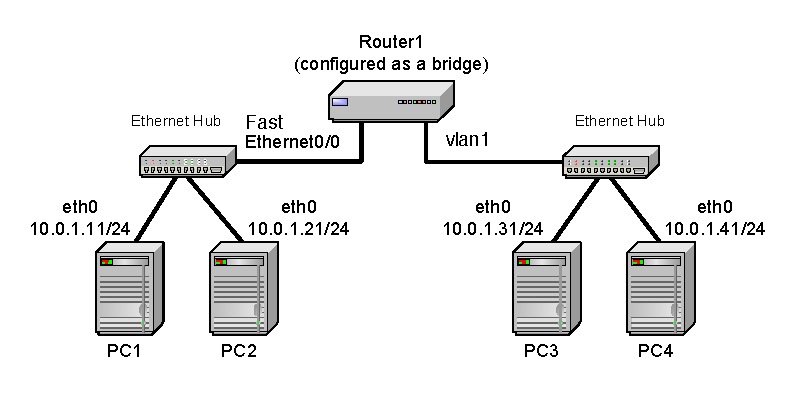
\includegraphics[width=\linewidth]{graphics/lab6-network2-updated.pdf}	
	\caption{Network Topology for Parts 2 and 3-b.}
	\label{fig:lab6-network2}
\end{figure}

\subsubsection{Exercise 2-a. Setup of network configuration}
After the network is configured, as in Exercise 1-a above for the Linux PCs, you are asked to record the MAC addresses of the Cisco routers.
\begin{enumerate}
	\item Connect the PCs and Router1 with Ethernet hubs as shown in Figure \ref{fig:lab6-network2}.
	\item Configure the \iface{eth0} interfaces of the Linux PCs with the IP addresses given in Table \ref{tab:lab6-network1}. (The IP addresses of PC1, PC2, and PC3 are the same as in Part 1). Disable the \iface{eth1} interfaces of all Linux PCs.
	\item Establish a \cmd{minimcom} session to each Cisco router: from PC1 to Router1, from PC2 to Router2, and so on.
	\item On each router, type \cmd{enable} and then use the command \cmd{show interfaces} to display the MAC addresses of the Ethernet interfaces. Record the MAC addresses in Table \ref{tab:lab6-macs-routers}.
		\begin{table}[h!t]
			\centering
			\begin{tabular}{| c | c | c |}	
				\hline
				\textbf{Linux PC} & \textbf{MAC address of FastEthernet0/0} & \textbf{MAC address of interface vlan1} \\ \hline
				Router1 & 00:0d:65:17:01:29 & 00:0d:65:17:01:29 \\ 
				Router2 & 00:0d:bc:ef:b1:a3 & 00:0d:bc:ef:b1:a3 \\
				Router3 & 00:0d:bc:ef:eb:24 & 00:0d:bc:ef:eb:24 \\
				Router4 & 00:0d:bc:ef:b9:48 & 00:0d:bc:ef:b9:48 \\ \hline
			\end{tabular}
			\caption{MAC addresses of the linux PCs}
			\label{tab:lab6-macs-routers}
		\end{table}
\end{enumerate}

\subsubsection{Exercise 2-b. Configuring a Cisco Router as a bridge}

Next you configure Router1 as a bridge. A Cisco router is configured as a bridge by disabling IP forwarding functions (with the command \cmd{no ip routing}) and by enabling bridging functions.

Similar as on the Linux PCs, a Cisco router can be configured to perform the functions of multiple independently operating bridges. This is done by defining a bridge group, which is identified by a number, and associating two or more network interfaces with each bridge group. Packets are forwarded only between interfaces that are assigned to the same bridge group. Since the exercises in Lab 6 only use one bridge group, we always use 1 to identify the group.

In order to create a bridge on the Cisco router, go into IOS's Global Configuration Mode and execute the following commands:
\begin{cmdblock}
	Router1(config)# bridge 1 protocol ieee
	Router1(config)# bridge 1 priority 128
\end{cmdblock}

The first command defines a bridge group identified by number 1 and assigns the spanning tree protocol as defined in IEEE 802.1d to bridge group 1. After the command is issued, the Cisco router forwards packets between all interfaces that are assigned to bridge group 1. A bridge group can be any number between 1 and 63. After defining a bridge group, one can assign network interfaces to the bridge group. It is possible to define multiple bridge groups. In Lab 6, only one bridge group (with identifier 1) is used.
The second command assigns the priority 128 to bridge group 1. The priority of a bridge group plays a role in the spanning tree protocol, which is covered in Part 5.

\boxinfo{Each interface is individually configured to participate in a bridge group. This is done with the following commands (all need to be run from the IOS Interface Configuration Mode):
	\begin{description}
		\item[\texttt{bridge-group 1}] \hfill \\
			Assign the current network interface to bridge group 1.
		\item[\texttt{no bridge-group 1}] \hfill \\
			Remove the current network interface from bridge group 1.
		\item[\texttt{bridge-group 1 spanning-disabled}] \hfill \\
			Disable the spanning tree protocol on the current interface for bridge group 1.
		\item[\texttt{no bridge-group 1 spanning-disabled}] \hfill \\
			Enable the spanning tree protocol on the current interface for bridge group 1.
	\end{description}
}

\boxinfo{Once a Cisco router is configured as a bridge, the following commands can be used to display the status of the bridge (all need to be run from the Privileged Exec IOS Mode):
	\begin{description}
		\item[\texttt{show bridge}] \hfill \\
			Display the entries of the MAC forwarding table.
		\item[\texttt{show spanning-tree}] \hfill \\
			Display the spanning tree topology information known to this bridge.
		\item[\texttt{show interfaces}] \hfill \\
			Display statistics of all interfaces, including the MAC addresses of all interfaces.
	\end{description}
}

\boxinfo{The following commands disable bridging functions on a Cisco router. The first must be executed in IOS's Global Configuration Mode, the subsequent commands must be run from the Privileged Exec IOS Mode):
	\begin{description}
		\item[\texttt{no bridge 1}] \hfill \\
			Delete the defined bridge group. After the command is issued, the Cisco router stops forwarding packets between interfaces that are assigned to bridge group 1.
		\item[\texttt{clear bridge}] \hfill \\
			Remove all entries from the MAC forwarding table.
		\item[\texttt{clear arp-cache}] \hfill \\
			Clear the ARP table.
	\end{description}
}

\begin{enumerate}
	\item Configure a Cisco Router as a Bridge: Use the above commands to configure Router1 as a bridge. On Router1, type the following commands:
		\begin{cmdblock}
	Router1> enable Password: <enable secret>
	Router1# configure terminal
	Router1(config)# no ip routing 
	Router1(config)# bridge 1 protocol ieee 
	Router1(config)# bridge 1 priority 128 
	Router1(config)# interface FastEthernet0/0 
	Router1(config-if)# bridge-group 1
	Router1(config-if)# bridge-group 1 spanning-disabled 
	Router1(config-if)# no shutdown
	Router1(config-if)# interface FastEthernet0/1 
	Router1(config-if)# no shutdown
	Router1(config-if)# interface vlan1 
	Router1(config-if)# bridge-group 1 
	Router1(config-if)# bridge-group 1 spanning-disabled 
	Router1(config-if)# no shutdown
	Router1(config-if)# end 
	Router1# clear bridge 
	Router1# clear arp-cache
		\end{cmdblock}
		The commands disable IP forwarding and set up Router1 as a bridge that runs with priority 128. Both Ethernet interfaces are assigned to the bridge, but the spanning tree protocol is disabled.
	\item Once Router1 has been configured as a bridge, configure the Linux PCs as shown in Figure \ref{fig:lab6-network1} with the IP addresses of Table \ref{tab:lab6-network1}.
	\item Delete all entries in the ARP caches of PC1 and PC3.
	\item Issue a ping command from PC1 to PC3.
		\begin{cmdblock}
	PC1% ping -c 1 10.0.1.31
		\end{cmdblock}
	\item Run \cmd{traceroute} from PC1 to PC3 and save the output. 
		\begin{cmdblock}
	PC1% traceroute 10.0.1.31
		\end{cmdblock}
\end{enumerate}

\begin{questions}
	\q{2.1}{Include the output of the \cmd{traceroute} command.}
	\q{2.2}{Compare the results to the outcome of the \cmd{traceroute} command in Exercise 1-c.}
	\q{2.3}{Why is it not possible to issue a \cmd{ping} command to Router1?}
\end{questions}

\newpage
\subsubsection{The Difference Between an Ethernet Hub and an Ethernet Switch}
In this part of the lab, you try to observe the difference between the operation of an Ethernet hub and an Ethernet switch. The main observation to be made is that traffic going over an Ethernet hub may experience collisions, whereas an Ethernet switch does not have collisions.

An Ethernet hub is a relatively simple device that merely repeats a signal received on one network interface (port) to all other ports. When multiple devices connected to the same hub transmit a packet at the same time, the transmissions are corrupted. This is referred to as a collision.

An Ethernet switch, which performs the functions of a bridge for Ethernet segments, is a store-and-forward device. When a packet is received, the Ethernet switch looks up the destination MAC address in its MAC forwarding table, and then forwards the packet to one of its ports. Transmissions on an outgoing link are done one packet at a time, and packets are buffered if multiple packets must be forwarded on the same output port at the same time.

In this context, dual-speed Ethernet hubs, which connect both 10 Mbps (10BaseT) and 100 Mbps (100BaseTX) Ethernet devices, are a special case. A dual-speed hub operates as two Ethernet hubs, one running at 10 Mbps and one running at 100 Mbps, that are connected by a bridge. Thus, there can be collisions between devices that operate at the same speed, but there are no collisions between devices at different speeds.

We point out that it is not always possible to observe collisions on an Ethernet hub. Not only does the rate of collision depend on the traffic load and pattern. In addition, hubs increasingly use internal buffering and avoid collisions in many cases.

\subsubsection{Exercise 3-a. Observe collisions on an Ethernet hub}
Try to generate collisions by flooding an Ethernet hub with traffic. The network configuration is as shown in Figure \ref{fig:lab6-network3}. You intentionally flood the hub that connects PC1 and PC2 with traffic and hopefully force collisions to occur.

\begin{figure}[h!t]
	\centering
	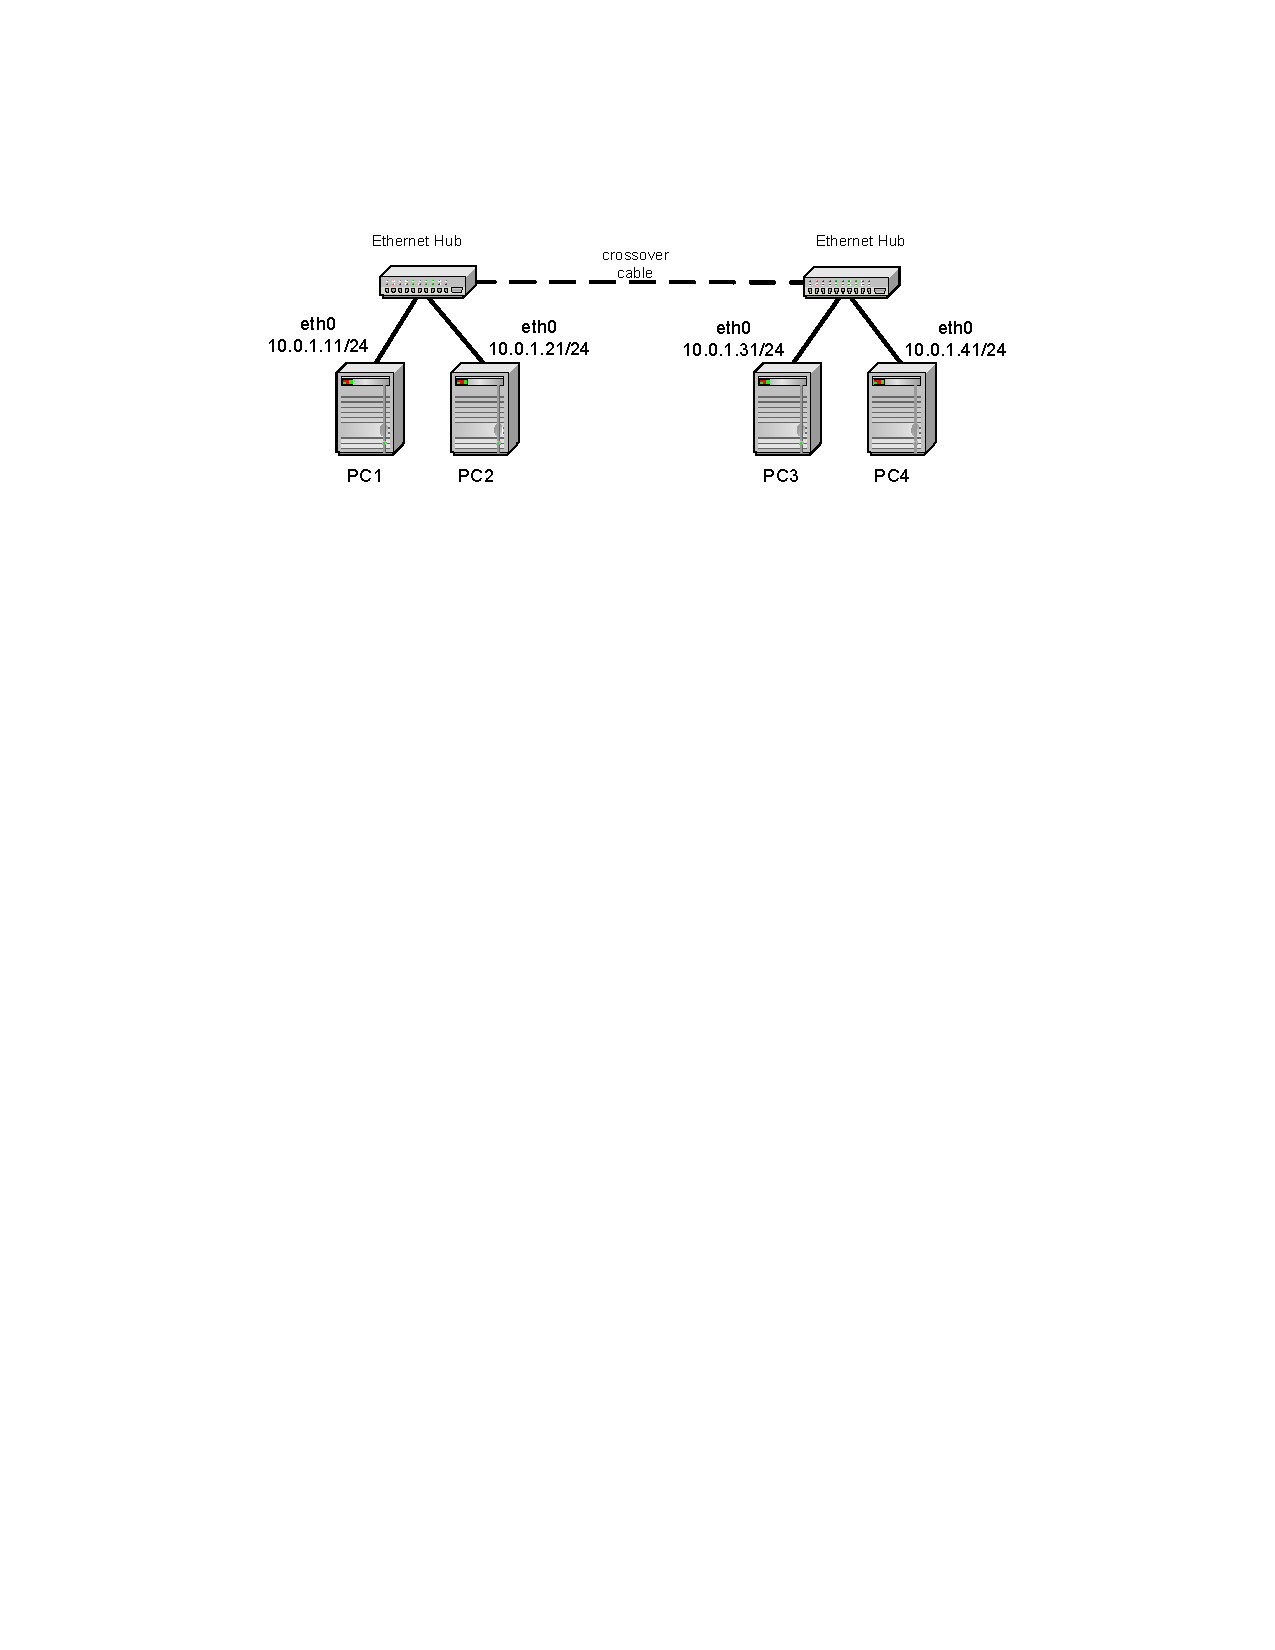
\includegraphics[width=\linewidth]{graphics/lab6-network3.pdf}	
	\caption{Network Topology for Part 3}
	\label{fig:lab6-network3}
\end{figure}

\begin{enumerate}
	\item Configure the network as shown in Figure \ref{fig:lab6-network3}. Starting from the network configuration from Part 2 (in Figure \ref{fig:lab6-network2}), disconnect Router1 and connect the two hubs directly with a crossover Ethernet cable (black cable, red RJ45 plugs).
	\item Determine the number of collisions on interface \iface{eth0} of PC1 and PC3, that have occurred since the PCs have been rebooted the last time, by typing
		\begin{cmdblock}
	PC1% ifconfig -a
	PC3% ifconfig -a
		\end{cmdblock}
		Save the output.
	\item Flood the network by generating a large number of ICMP Echo Request and Reply packets between PC1 and PC2, by typing
		\begin{cmdblock}
	PC1% ping -f 10.0.1.21
		\end{cmdblock}
	\item While the above ping command is running, start sending 100 ICMP Echo Request packets from PC3 to PC4.
		\begin{cmdblock}
	PC3% ping -c 100 10.0.1.41
		\end{cmdblock}
		Hopefully, these ping messages cause some collisions at the Ethernet hub.
	\item On PC1 and PC3, save the output of \cmd{ifconfig -a} again. Observe the number of new collisions that the above experiment has generated.
\end{enumerate}

\begin{questions}
	\q{3.A}{Calculate the number of new collision as seen by PC1 and PC3, in the above exercise. Briefly explain what causes the collisions.}
\end{questions}	

\subsubsection{Exercise 3-b. No collisions when using an Ethernet switch}
Repeat the steps of the previous exercise, but place an Ethernet switch (Router1, which has been configured as a bridge), between the two Ethernet hubs.

\begin{enumerate}
	\item Reconstitute the network configuration shown in Figure \ref{fig:lab6-network2}, by connecting Router1 between the two hubs.
	\item Obtain the number of collisions that have been observed on interface \iface{eth0} of PC1 and PC3 by typing
		\begin{cmdblock}
	PC1% ifconfig -a
	PC3% ifconfig -a
		\end{cmdblock}
		Save the output.
	\item Flood the network with traffic by generating a large number of ICMP Echo Request and Reply packets between PC1 to PC2, by typing 
		\begin{cmdblock}
	PC1% ping -f 10.0.1.21
		\end{cmdblock}
	\item Now issue 100 ICMP Echo Request packets from PC3 to PC4: 
		\begin{cmdblock}
	PC3% ping -c 100 10.0.1.41
		\end{cmdblock}
	\item Once again, save the output of the command \cmd{ifconfig -a} on PC1 and PC3, and record the number of collisions on interface \iface{eth0}.
	\item Access Router1 and run the \cmd{show bridge} command to display the bridge forwarding table. Save the data.
\end{enumerate}

\begin{questions}
	\q{3.B}{Use the \cmd{ifconfig -a} output to calculate the new collisions seen at the interfaces of PC1 and PC3. Explain the differences between the outcomes in Exercise 3-a and Exercise 3-b.}
\end{questions}
	
\newpage
\subsection{Learning Bridges}

Each bridge has a MAC forwarding table that determines the port where a packet is transmitted from. When a packet arrives, the bridge looks up the destination MAC address of the packet in its MAC forwarding table, and retrieves the outgoing port for this packet. If the destination MAC address is not found in the forwarding table, the bridge floods the packet on all ports, with exception of the port where the packet arrived.

Bridges update their MAC forwarding table using what is called a learning algorithm, which works as follows. A bridge examines the source MAC address of each packet that arrives on a particular port, and memorizes that the source address is reachable via that port. This is done by adding the source MAC address and the port to the MAC forwarding table. The next time the bridge receives a packet which has this MAC address as destination, the bridge finds the outgoing port in its forwarding table. Bridges that run this algorithm are referred to as learning bridges. All currently deployed Ethernet switches execute the learning algorithm.

An entry in the MAC forwarding table is deleted if it is not used (looked up) for a certain amount of time. The maximum time that a MAC address can stay in the forwarding table without a lookup is determined by the \emph{Ageing} value, which is a configuration parameter.

Here you investigate the learning algorithm of bridges. The network configuration is as shown in Figure \ref{fig:lab6-network4}.

\begin{figure}[h!t]
	\centering
	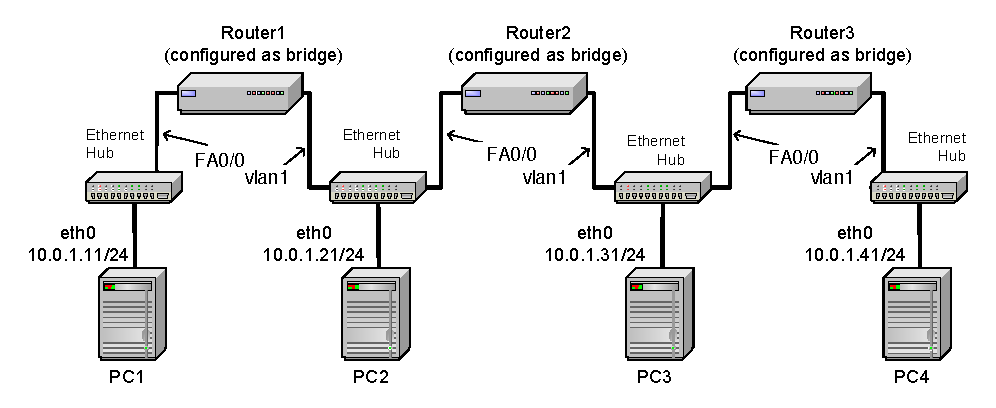
\includegraphics[width=\linewidth]{graphics/lab6-network4-updated.pdf}	
	\caption{Network Topology for Part 4}
	\label{fig:lab6-network4}
\end{figure}

\subsubsection{Exercise 4-a. Exploring the learning algorithm of bridges}

In this exercise you study how bridges set up their MAC forwarding tables from the network traffic.
\begin{enumerate}
	\item Set up the network configuration as shown in Figure \ref{fig:lab6-network4}.
	\item Establish a \cmd{minicom} session to Router1, Router2, and Router3.
		\begin{itemize}
			\item Configure Router1, Router2, and Router3 as bridges (Disable the spanning tree protocol).
			\item On each of the bridges, delete the contents of the MAC forwarding table with the \cmd{clear bridge} command.
		\end{itemize}
	\item Verify that PC2 is not running as a bridge. If necessary, follow the instructions in Exercise 1-d to disable the bridging functions on PC2. Also, verify that on each PC only interface \iface{eth0} is enabled.
	\item Start to capture traffic with ethereal on the \iface{eth0} interfaces of PC1, PC2, PC3, and PC4.
	\item Clear the ARP cache on PC1, PC2, and PC3.
	\item Now, issue a set of \cmd{ping} commands. After each command, save the MAC forwarding table on all bridges with the command show bridge, and observe how far the ICMP Echo Request and Reply packets travel.
		\begin{cmdblock}
	PC1% ping -c 1 10.0.1.21 
	PC2% ping -c 1 10.0.1.11 
	PC2% ping -c 1 10.0.1.41 
	PC3% ping -c 1 10.0.1.21
		\end{cmdblock}
	\item Stop the traffic capture on the PCs, and save the ethereal output.
\end{enumerate}

\begin{questions}
	\q{4.A.1}{ Use the captured data to illustrate the algorithm used by bridges to forward packets.}
	\q{4.A.2}{For each of the transmitted packets, explain if the learning algorithm results in changes to the MAC forwarding table. Describe the changes.}
\end{questions}

\subsubsection{Exercise 4-b. Learning about new locations of hosts}

Learning bridges adapt their MAC forwarding tables automatically when the location of a host changes. Due to the learning algorithm, the time it takes to adapt to a change depends on the network traffic and on the value of the Ageing parameter. This is illustrated in the following exercise.

\begin{enumerate}
	\item Continue with the configuration of the previous exercise. First, create or refresh entries in the MAC forwarding table at the bridges by issuing the following commands from PC1:
		\begin{cmdblock}
	PC1% ping -c 3 10.0.1.31 
	PC1% ping -c 3 10.0.1.41
		\end{cmdblock}
	\item Now, connect PC2 to the same hub that PC4 is connected to.
	\item Issue a ping command from PC1 that continuously sends ICMP Echo Request packets to PC2
		\begin{cmdblock}
	PC1% ping 10.0.1.21
		\end{cmdblock}
		Since Router2 does not know that PC2 has moved, it does not forward the ICMP Echo Request packet, and packet does not reach PC2. As a result, the ARP requests and the ping are unsuccessful. Eventually, since the MAC forwarding entry for PC2 is not refreshed at Router2 and Router3, the entry is deleted. When the entry is removed, the next ICMP Echo Request from PC1 is flooded on all ports, thus reaching PC2. When PC2 responds, all bridges update their MAC forwarding table using the source MAC address of PC2.
		Record the amount of time that the ping from PC1 to PC2 is not successful after PC2 has been moved to a different hub.
	\item Now connect PC3 to the same hub as PC4.
	\item Issue a \cmd{ping} command from PC1 to PC3 that continuously sends ICMP Echo Request packets to PC3: 
		\begin{cmdblock}
	PC1% ping 10.0.1.31
		\end{cmdblock}
	\item Then, generate a single ICMP Echo Request packet from PC3 to PC1 with the command
		\begin{cmdblock}
	PC3% ping -c 1 10.0.1.11
		\end{cmdblock}
		Now, if you look on PC1, you notice that the \cmd{ping} command is successful again. Explain this outcome and compare it to the outcome of Step 2.
\end{enumerate}

\begin{questions}
	\q{4.B.1}{Include the times that you recorded in Steps 3.}
	\q{4.B.2}{Explain the outcome of Step 6. That is, explain why the ping issued by PC3 has the effect that the ping commands from PC1 to PC3 (in Step 5) are successful. Compare the outcome with the outcome in Step 3.}
\end{questions}
